
\documentclass[DIV=calc,paper=a4,fontsize=9pt,twocolumn]{scrartcl}
\renewcommand*\sfdefault{lcmss}
\renewcommand*\familydefault{\sfdefault} 
\usepackage[T1]{fontenc}

\usepackage{lipsum}                                                 
\usepackage[utf8x]{inputenc}
\usepackage[english]{babel}								
\usepackage[protrusion=true,expansion=true]{microtype}	
\usepackage{amsmath,amsfonts,amsthm}					
\usepackage[pdftex]{graphicx}							
\usepackage[svgnames]{xcolor}							

\usepackage{epstopdf}									
\usepackage{subfig}										
\usepackage{booktabs}									
\usepackage{fix-cm}										
\usepackage{csquotes}
\usepackage[authoryear,round]{natbib}
\usepackage{float}
\usepackage{url}
\bibliographystyle{apalike}
\definecolor{headblue}{HTML}{15778E}
\definecolor{borderblue}{HTML}{074C5C}


\usepackage{sectsty}		
							
\allsectionsfont{\usefont{OT1}{phv}{b}{n}}				
														

\sectionfont{\usefont{OT1}{phv}{b}{n}}					
														




\usepackage{fancyhdr}									
    \pagestyle{fancy}									
\usepackage{lastpage}   


\lhead{}
\chead{}
\rhead{}

\lfoot{\footnotesize 2013 \textbullet ~ Tools and Evaluation Methods used in Open Source Development}
\cfoot{}
\rfoot{\footnotesize page \thepage\ of \pageref{LastPage}}  
\renewcommand{\headrulewidth}{0.0pt}
\renewcommand{\footrulewidth}{0.4pt}




\usepackage{lettrine}
\newcommand{\initial}[1]{
     \lettrine[lines=2,lhang=0.3,nindent=0em]{
                    \color{headblue}
                    {\textsf{#1}}}{}}




\usepackage{titling}										

\newcommand{\HorRule}{\color{headblue}\rule{\linewidth}{1pt}}

\pretitle{\vspace{-30pt} \begin{flushleft}  \fontsize{30}{30} \usefont{OT1}{phv}{b}{n} \color{borderblue} \selectfont }
\title{Tools and Evaluation Methods used in Open Source Development}    
\posttitle{\par\end{flushleft}\vskip 0.5em}

\preauthor{\begin{flushleft} \large \usefont{OT1}{phv}{b}{sl} \color{headblue}}
\author{Steffen Tröster \\}											
\postauthor{\footnotesize \usefont{OT1}{phv}{m}{sl} \color{Black} 
                    University of Tampere, 2013							
                    \par\end{flushleft}\HorRule}

\date{}																




\begin{document}
\maketitle
\thispagestyle{fancy}		

\initial{O}ne says that the open source paradigm is one of the most promising strategies to improve the quality and efficiency of software development processes. This essay is introducing into the approach and methodologies of open source, its software development model and its use of software engineering tools during the processes.

It will also review some evaluation models and a framework to choose the right evaluation model for the specific need. After this introduction it will give an example how to introduce automated quality assurance with an open source project based on NodeJS technologies and established with continues integration. 

\section{Introduction}

The open source software development paradigm is one of the most upcoming way of new software development. Software developed in this way is free in use, spreading and contribution with the condition of continuing the open source paradigm. But this alleged \enquote{free} results out of open source development processes are nearly all commercial projects which are raising money with different service offers \citep{Wheeler}. That means that a usual open source developer usual is paid by companies to develop on open source software, to improve the product so that these companies can offer well paid services like hosting or support for this product. Others which are contributing are doing it because of their personal need.

To ensure a proper result in open source development with all different co-developer, from an established community, there should be a sharp regulation progress for input and iterations. Also difficult is the opportunity to develop from all over the world. Therefor the open source development paradigm uses a set of different software engineering tools with features which helps in given cases like collaboration, status-tracking and testing.

\enquote{To a large extent, the open source culture and methodology are conveyed to new developers via the toolset itself, and through the demonstrated usage of these tools on existing projects.} \citep{Robbins02adoptingoss}

There are different indicators why open source is one of the most promising strategies to improve the quality and efficiency of software development processes. The first one is that projects have a huge crowd of individual users who are willing to contribute to a project by different impulsions. This causes fresh ideas and resources from different minded developer from different cultures. Thats why companies are more and more focusing on the open source approach. They can successfully develop bigger projects by involving the community. But also public institutions like schools or city administrations are as even interested on this approach. Open Source can form more security, safety and trustworthiness in this division because everyone can check and view the used systems. The last indicator are popular and successful products like \enquote{Linux} and \enquote{Apache} which are gaining more and more leading shares in their own markets. \citep{fuggetta2003open}

\subsection{Open Source Software Development Model}

Next to the given toolset, there is an open source development model which is characterized by processes and values of a different kind as traditional proprietary development models. This model takes a new approach for more fluidly development by increasing collaboration, continuous integration and testing. It also involves the end-users deeper into design decisions. Some companies may use a slightly modified version of this model depending on their claims. \citep{Haddad11}

The Model in Figure \ref{fig:feature-life-cycle} shows a typical feature life-cycle. A feature request is coming from the user or developer community of the project by mailing list or issue tracker. It will discussed in the whole community and results to an architecture or design decision which is received into an implementation process if it is accepted. After the implementation the new feature will be verified by continuous integration and (automated) testing. This whole process is iteration based and can flow back to the decision process to ensure a necessary project quality when for example a testing of a feature failed or when it contradicts other design decisions. After a successfully testing the feature will be deployed in a new project version and can be maintained by the user and development community. \citep{Haddad11}

\begin{figure*}[ht]
    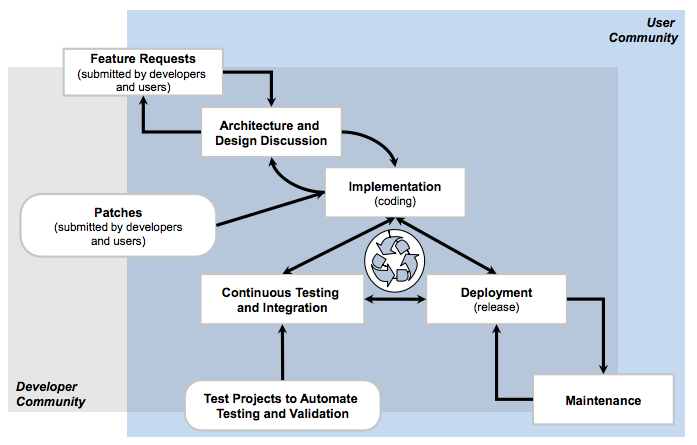
\includegraphics[width=0.8\textwidth ]{img/feature-life-cycle.png}{}
    \centering
    \caption{Feature life-cycle in the open source development model. \citet{Haddad11}}\label{fig:feature-life-cycle}
\end{figure*}

\section{Tools in Open Source Software Development}

Software Engineering tools which are created and used in open source software development are fitting to the different processes of the given software development model. These tools are widely the result of daily practices so that they carry support for the given use cases in open source software development. \citep{Robbins02adoptingoss} 

Back to the model of \citet{Haddad11}, each process is constituting a special type of tool. First of all communication tools are important to contribute feature requests, issues and bugs to a project. These tools are also used to make the design decisions in the developer and user community. The second topic of tools are version control systems and collaboration tools to facilitate parallel contribution from all over the world. The software need to be tested according to the given open source model after contribution. Therefor a toolset of different testing and continues integration tools are available. They will be discussed in the following sub chapters.

\subsection{Communication - Issue and Bugtracking}

The most important action, which is done in every process of the open source software development model is communication. Almost every project is using mailing lists to discuss design decisions and new features and approaches with the developer and user community. Some projects are using asynchronous communication like IRC in addition, but it is still a more or less organized communication process. Next to these direct communication techniques, there are also the projects specific websites, FAQ's and Wikis in use to communicate news and important information about the project to users which are not participating in the current development. \citep{ApacheFoundation13} 

An even more organized communication are offering issue-tracker or ticket-systems like \enquote{Bugzilla} or the \enquote{GitHub Issue-Tracker}. With those trackers it is possible to collect a lot of information from users and developers about bugs, reports, features and ideas and they offer also a way to rate or prioritize them. The prioritisation can also be done by issue ratings, commenting and \enquote{pushing} which is the process of raising the urgency of an issue. After a decision is made by the community each report can be assigned to a specific developer or group which is solving or implementing the made design decision after an issue.

\subsection{Version Control and Collaboration}

How to enable people from all over the world to collaborate on one specific open source project at the same time? Version control systems are the most important tools during the implementation phase of the open source software development model. This tools offer every developer to contribute new code, files and documentation for the given project by merging them with other contributions. 

In the beginning of open source project centralized version control systems like \enquote{Subversion} or \enquote{Concurrent Versions System} where widely in use and were over the years replaced by distributed version control systems like \enquote{Git}. \citet{rodriguez2012distributed} are saying that this change to distributed system is giving a lot of advantages. Every developer has now a local development version where he can commit new changes as changeset. Versions are not anymore saved as single file per version but as changeset, which can be merged into every further version. Hence every developer can work on different versions without merging every commit from others in order to contribute to the project.

This new technology reduces also the barriers for non-core developers of an open source project which can contribute without being connected to a central or remote repository which further need to be established and approved. They can simply suggest a changeset to a project which can be merged after reviewing. The contributer will be invited to the core developers if there is a big potential visible. This advantage improves every open source project with new ideas and manpower. Condensed it is easier to get part of developer communities of open source projects. \citep{rodriguez2012distributed}

\subsection{Testing and Continues Integration}

Automated testing and continues integration are the first steps to a predefined quality assurance during the development process. With automated testing it is possible to test functional and non-functional requirements by coded tests. Those tests can handle different application layers beginning on unit tests which test single components of software. Integration tests are testing the interfaces between the components of software. System Tests are testing every software component in a completed and integrated system. The last layer acceptance tests are evaluating the system's agreement with the business requirements whether it is acceptable for delivery. \citep{abran2001guide}

With continues integration are integration problems between software modules during the process and thereby earlier found. In addition to distributed version control systems can this also be a good validation in order to verify a new contribution request with new code changesets. They can be tested before they are merged in the main project through continues integration. Another advantage is that there is also always a running system for demo, testing or distribution purpose available.

\section{Evaluation Models for Open Source Software}

There are two major concerns of open source software evaluation. The first concern is the evaluation to ensure a specific open source software quality of a companies or communities product during the open source software development process. 

Next to the software quality evaluation there are also different evaluation methods to support decisions for using a specific system. Often a company searches for open source product to solve a given issue and there are more than one solution available that solves the issue. Since the quality of open source software products varies widely, a company which want to use a specific product need to decide which is the best available open source system \citep{stol2010comparison}. There are more than 20 evaluation models available for this purpose. They are listed in a research paper of \citet{stol2010comparison}.

This essay will review respective one of the major concerts. First the Selection Process of Open Source Software by \citet{lee2007study} and than the Source Quality Observatory for Open Source Software (SQO-OSS) by \citet{samoladas2008sqo}.

\subsection{Selection Process of Open Source Software}

The Selection Process of Open Source Software is focusing on offering a specified method to compare different open source solutions for a given issue or problem in companies. Because it is often difficult to identify the target open source software which is satisfying the systems requirements among all other open source projects. \citep{lee2007study}

\enquote{Without a formal methodology that implements a standardized analytical framework, organizations are limited in their ability to assess the maturity of a product.} \citep{golden08}

\begin{figure}[ht]
    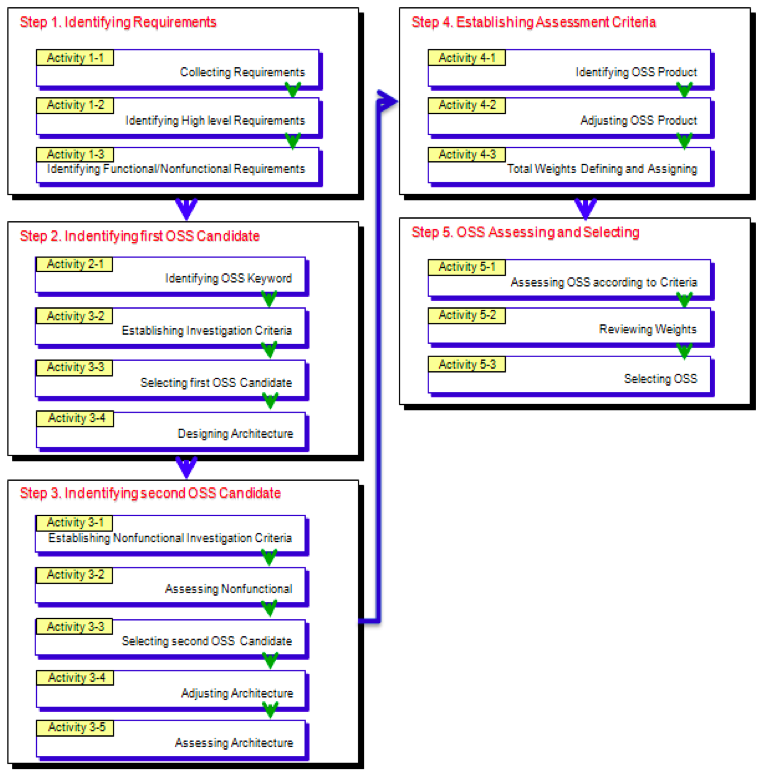
\includegraphics[width=0.5\textwidth ]{img/selectionprocess.png}{}
    \centering
    \caption{Selection Process of OSS. \citet{lee2007study}}\label{fig:selection-process.png}
\end{figure}

\citet{lee2007study} are saying that although it is possible to identify some open source systems satisfying requirements, there isn't a variety specification to gain. This is because this system communities doesn't provide product or project information for analyzing and comparing. Hence these step cause many trials and errors and there is a need to solve these problems.


The selection process shown by \citet{lee2007study} is based on five steps with some sub actions, which can be seen in Figure \ref{fig:selection-process.png}:

\begin{enumerate}
    \item Identifying Requirements: What requirements are required by the open source system to solve the companies problem and reach its goal?
    \item Identifying first OSS candidates: By selecting keywords out of the requirements, the first candidates can be selected by searching for this keywords and given conditions like running platform or used programming language.
    \item Identifying second level OSS candidates: Searching for exceptions and quality requirements in the not functional requirements to restrict the choice of first level open source software candidates.
    \item Establishing Assessment Criteria: This step identifies open source software candidates and arranges to evaluate them, and decides weight on detailed function of each module and maps candidates to prepare for evaluation.
    \item OSS Assessing and Selecting: This step carries out an evaluation of the selected open source systems which will be used for the given issue. 
\end{enumerate}

To ensure a specific software quality of the given information system an evaluation method in the last two steps is necessary. In the following part a automatic software quality assurance evaluation with specified metrics is reviewed. This evaluation method can also be used in the step number \enquote{4. Establishing Assessment Criteria} of this methodology.

\subsection{Source Quality Observatory for Open Source Software}\label{sec:sqsoss}

The SQO-OSS model by \citet{samoladas2008sqo} is focusing on automated software quality assurance. This enables an automatic metrics collection approach and thereby a continuous quality monitoring system can be established which can be seen in Chapter \ref{sec:automated-quality-assurance}. It also takes the community factors into account if only those community factors that can be measured automatically. These factors are also mainly focusing on the fundamental aspects of open source software quality like the project maintainability, reliability and security. 

\begin{figure}[ht]
    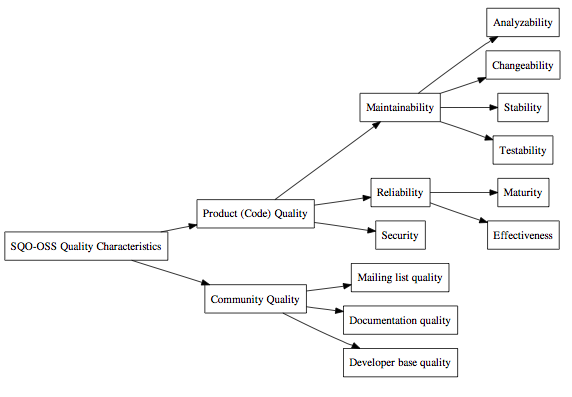
\includegraphics[width=0.5\textwidth ]{img/sqsoss.png}{}
    \centering
    \caption{The SQS-OSS quality model. \citet{samoladas2008sqo}}\label{fig:sqs-oss}
\end{figure}

This model is subdividing every criteria of software quality until it is automatically measurable by analyzing source code factors and community attributes. Figure \ref{fig:sqs-oss} is showing the different hierarchy of quality criteria with each subdivision for the specific measurement. The both main criteria for open source software quality are the actual product quality and the covered community quality. These two main factors recur also in chapter \ref{sec:oss-success} about the open source software success evaluation.

Automatic measurable metrics defined by \citet{samoladas2008sqo} for the criteria changeability are for example: average size of statements, vocabulary frequency, number of unconditional jumps, number of nested levels, coupling between objects (CBO), lack of cohesion (LCOM) and depth of inheritance tree (DIT). On the community side the metrics of the criteria maturity are for example: number of open critical bugs in the last 6 months and number of open bugs in the last six months. The measurement for this criteria are quantified in the following four terracing categories Excellent (E), Good (G), Fair (F) and Poor (P). \citep{samoladas2008sqo}

\subsection{Comparison Framework for Open Source Software Evaluation Methods}

Now the important question is, how to choose between all the different evaluation methods. \citet{stol2010comparison} have already shown the 20 different evaluation methods. They also show if these method comes from industry or research and if it provides a predefined methodology for applying or not. They are also saying that the specific approach is more and more depending on the needed information and subject of scope for a needed evaluation.

Next to these information \citet{stol2010comparison} are also offering a framework to compare these evaluation methods. They call it Framework fOr Comparing Open Source Software Evaluation Methods (FOCOSEM). The following list of criteria to characterize a evaluation technique is a short overview of this Framework:

\begin{enumerate}
    \item Method Context
    \begin{enumerate}
        \item Specific goal: What is the particular goal of the method?
        \item Functionality evaluation: Is functionality compliance part of the evaluation method?
        \item Results publicly available: Are evaluations of OSS products stored in a publicly accessible repository?
    \end{enumerate}
    \item Method User
    \begin{enumerate}
        \item Required skills: What skills does the user need to use the method?
        \item Intended users: Who are the intended users of the method?
    \end{enumerate}
    \item Method Process
    \begin{enumerate}
        \item Method's activities: What are the evaluation method's activities and steps? 
        \item Number of criteria: How many criteria are used in the evaluation?
        \item Evaluation categories: What are the method's categories of criteria based on which the OSS product is evaluated?
        \item Output: What are the outputs of the evaluation method?
        \item Tool support: Is the evaluation method supported by a tool?
    \end{enumerate}
    \item Method Evaluation
    \begin{enumerate}
        \item Validation: Has the evaluation method been validated?
        \item Maturity stage: What is the maturity stage of the evaluation method?
    \end{enumerate}
\end{enumerate}

\citep{stol2010comparison}
\\

\enquote{We note that the objective of FOCOSEM is not to make any judgments about different OSS evaluation methods. Instead, we aim to provide insights that may help practitioners to select a suitable OSS evaluation method.} \citep{stol2010comparison} It should also help to understand the aspired goal of an analyzed evaluation method. 

\subsection{Open Source Software Success} \label{sec:oss-success}

An other way of evaluation is measuring the success of open source software projects which is already done by some studies and researches which are mostly qualitative or exploratory in nature. This evaluation of open source software success is important for future project improvements because statistics are showing that 58\% of projects in Sourceforge, which is a open source project host, since 2005 where failing. 

\citet{lee2009measuring} have developed a model to identify five determinants for open source software success as well as a number of significant relationships between them. They extended the \citet{delone1992information} success framework for information systems in respect of its updates by \citet{seddon1997respecification} and them self ten years later in scope of open source software development. They applied the information system success model to the open source software context and found that the OSS success model shared similarities and differences with other contexts. \citep{lee2009measuring}

The model in figure \ref{fig:success-model} is showing the the five determinants: software quality, community service quality, user satisfaction, open source software use, and individual net benefits and the positive influence of each other (arrows with H*). With their research they are demonstrating that software quality and community service quality have decisive effects on user satisfaction. \citep{lee2009measuring}

\begin{figure}[ht]
    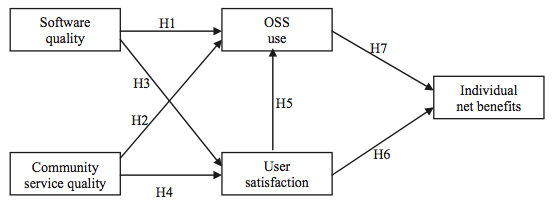
\includegraphics[width=0.5\textwidth ]{img/success-model.png}{}
    \centering
    \caption{Extended research model by \citet{lee2009measuring}}\label{fig:success-model}
\end{figure}

\enquote{Software quality and user satisfaction, in turn, have significant effects on OSS use. Additionally, OSS use and user satisfaction have significant effects on individual net benefits.} \citep{lee2009measuring}

\section{Automated Quality Assurance}\label{sec:automated-quality-assurance}

This chapter will deal with an approach for automated quality assurance. I personally think that an automated quality assurance process can be established in every open source project during the testing and/or continues integration. I'm going to show this example approach with a project which is called georeport which is going to become a nodeJS based open311 georeport v2 API implementation. That means the project just started and is currently under development so that a automated quality assurance system could come quite handy. This project is available on GitHub and can be found at https://github.com/stetro/georeport.

The aim of the georeport project is to develop an open source solution for servers to provide a simple HTTP REST based open311 interface. This open standard open311 is a standard specification for a collaborative civic issue tracking which is already in use in several cities in US and EU like Helsinki and it is also going to be used in Tampere in the future. \citep{open311}

\citet{van2002java} are saying that software inspection is a well known technique for improving the software quality. This method is traditionally a formal process that involves analysts with manual analysis techniques such as formal code reviews and structured walk-through. This inspection is a specified and systematic process which is mostly well guided and defined. Therefor there are a lot of analytic tools available to automate this process. Next to the described source analytics to find code smells in projects as explained by \citet{van2002java} there is the possibility to expand this approach to social factors of software quality and quality of open source software as it is earlier described in the SQO-OSS quality model of chapter \ref{sec:sqsoss} by \citet{samoladas2008sqo}.

In the first part a possible product quality assurance will be shown. After this an example of community quality assurance will also be presented.

\subsection{Product Quality}

NodeJS and the associated package control manager \enquote{npm} offer a lot of open source modules for measuring code complexity and quality with different approaches. Such modules are for example \enquote{jslint}, \enquote{escomplex} and \enquote{jscheckstyle}. The most significant analyze module in view of code complexity is given by escomplex. It consists out of different analytic tools developed in NodeJS. These modules are based on different research approaches for measuring complexity or maintainability such as \enquote{A Complexity Measure} by \citet{mccabe1976complexity} or \enquote{Cyclomatic Complexity Density and Software Maintenance Productivity} by \citet{gill1991cyclomatic}.

Testing in general is realized with the \enquote{mocha} library for different test types like unit or integration tests for NodeJS. In those tests there is as usual a before or beforeEach instruction to configure a specific testing environment. Now there can be also a source quality analytic added. The following tests can be coded in the style of an usual unit test by using the escomplex library. The before statement used in this test is loading every source file and is also measuring the source quality and complexity with this library. In the following tests there can be an average or every file result be tested. The actual used product quality test for this project can be found in the GitHub project of georeport.

The used Metrics in escomplex for measuring the code quality and complexity are the following:

\begin{enumerate}
    \item Number of parameters: Is analyzing the amount of function parameter. Lower is better.
    \item Cyclomatic complexity: This Metric is defined by \citet{mccabe1976complexity} and its a count of the number of cycles in the program flow control graph. Effectively the number of distinct paths through a block of code. Lower is better.
    \item Halstead metrics: This Metric is defined by Maurice Halstead in 1977 \citep{zuse2005resolving} and they are calculated from numbers of operators and operands in each function. Lower is better.
    \item Maintainability index: This Metric is defined by \citet{oman1992metrics} and it is a logarithmic scale from negative infinity to 171, calculated from the logical lines of code, the cyclomatix complexity and the Halstead effort. Higher is better.
    \item Dependencies: This metric is counting the use of JavaScript require method to make a new library dependency. Lower is better.
    \item First-order density: The percentage of all possible internal dependencies that are actually realized in the project. Lower is better.
    \item Change cost: The percentage of modules affected, on average, when one module in the project is changed. Lower is better.
    \item Core size: The percentage of modules that are both widely depended on and themselves depend on other modules. Lower is better.
\end{enumerate}

\citep{escomplex2013}

\subsection{Community Quality}

Next to the product quality metrics as shown below it is also possible to measure community attributes on GitHub. The project host GitHub is offering a huge API where everyone can interact with to create own tools which improve the open source software development work flows. Next to the management tasks and resources which are offered by this API there are also a lot of informations to measure the community quality in the way of SQS-OSS model. \citep{githubAPI2013}

To get access to the API GitHub also offers a list of own or third party libraries for every different programming language and technology stack. This library, called Octocat, is also available for node (octonode) and it is possible to gather these following SQS-OSS attributes:

\begin{enumerate}
    \item Counting critical issues, bug fixings and overall issues of the last several month to ensure project activity and project maturity. 
    \item Analyzing the developer base with counting the project subscriber, star giver, collaborators and project contributers.
    \item Development activity is also measured by counting the last commits and commits of the last several days.
\end{enumerate}

This way of measuring can still be extended by using statistic measuring and analyzing values over a certain time period to consider the evolution of this project. 

\subsection{Automation}

The georeport project is as TravisCI project established. Every time someone is doing a commit to the project the continues integration services TravisCI is taking the whole project from GitHub and is running every available test in this project to ensure that is still valid with respect to the given tests. As we think about the quality tests described before, they can also be run every single time someone committed something new to the project. May the problem with this approach is that the whole project build fails when a single quality test fails. May there should be a separate state to show the status of \enquote{Quality Assured}.

\section{Conclusion}

The open source software development paradigm is one of the most upcoming way of new software development. But it is not about free software, its the idea of collaborating and giving the project the chance to get contributed by new ideas from programmers with different culture and needs. The used tools such as communication tools, version control tools and testing tools are the fundamental pieces to ensure this approach of collaborative work.

To benefit as user of open source software by this approach of open source development these huge amount of upcoming new software still need to be evaluated. Evaluation can be done to ensure that a searched open source product comes close to the actual needs of a given use case or to ensure product quality in view of maintainability, security and reliability. To carry out this evaluation \citet{stol2010comparison} showed us about 20 evaluation frameworks and also a framework to compare and choose the right one for a specific need.

Another important evaluation is the success analysis for information systems by \citet{delone1992information}. This model and also the newer version developed by them self ten years later is strongly context based and does not fit into the open source software scope. Thats why there was a need for a new model which is developed by \citet{lee2009measuring} who was revising the models by \citet{delone1992information} to the open source approach.

In the last part of this essay I tried to establish an example of testing, continues integration and automated quality assurance in a NodeJS based open source product called georeport.

\bibliography{library}

\end{document}
